\documentclass[12pt]{standalone}

\usepackage{tikz}
\usepackage{ctex}

\begin{document}
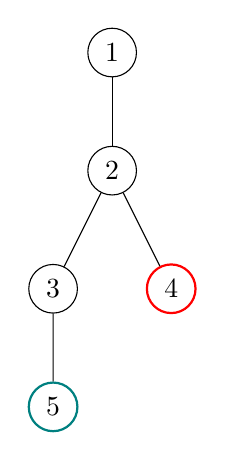
\begin{tikzpicture}

% the tree

\begin{scope}[circle,every node/.style={draw}]
    \node at (0,0) {$1$}
        child {node {$2$}
            child {node {$3$}
                child {node[draw=teal,thick] {$5$}}}
            child {node[draw=red,thick] {$4$}}};
\end{scope}

% the stack (not shown in this diagram)

%\begin{scope}[draw,minimum height=6mm,minimum width=1.5cm]
%    \node[draw=teal] at (4cm,0mm) {$1$};
%    \node[draw=red] at (4cm,-12mm) {$2$};
%\end{scope}

%\draw[->] (4cm,-8mm) -- (4cm,-4mm);

\end{tikzpicture}
\end{document}
